\chapter{Test Journal: Controllers Implementation} \label{app:ModelNode}

\textbf{Date: 25/05/2017}

\subsection*{Purpose}
Check the performance of the inner and outer controller code, when tested with a ROS node that simulates the dynamics of the vessel.

\subsection*{Equipment}
\begin{itemize}
    \item Vessel with all its components. 
    \item External laptop.
\end{itemize}

\subsection*{Procedure}
\begin{enumerate}
    \item Turn on all equipment.
    \item Remotely log into the boat, when both, laptop and vessel's computer, are in the same network.
    \item Run the following nodes
    \begin{itemize}
        \item \lstinline[style=cinline]{/lqr_node}  
        \item \lstinline[style=cinline]{/model_node}
    \end{itemize}
    \item Record the following topics
    \begin{itemize}
        \item \lstinline[style=cinline]{/kf_attitude}
        \item \lstinline[style=cinline]{/kf_position}   
        \item \lstinline[style=cinline]{/lli_input}  
    \end{itemize}
    \item Run the following topic with a step in $\dot{x}_\mathrm{b}$/$\psi$.
    \begin{itemize}
        \item \lstinline[style=cinline]{/controller_node}
    \end{itemize}
    \item Stop the recording after some time has passed.
    \item Repeat from 3 but including the \lstinline[style=cinline]{/path_follower_node}.
    \item Process the data.
\end{enumerate}

\subsection*{Results}
The result of the implemented code are shown below
\begin{figure}[H]
    \captionbox  
    {  
        Step response in $\psi$ of the implemented controller code for the inner controller together with the model node.
        \label{fig:model_node_yaw}                                
    }                                                                 
    {                                                                  
        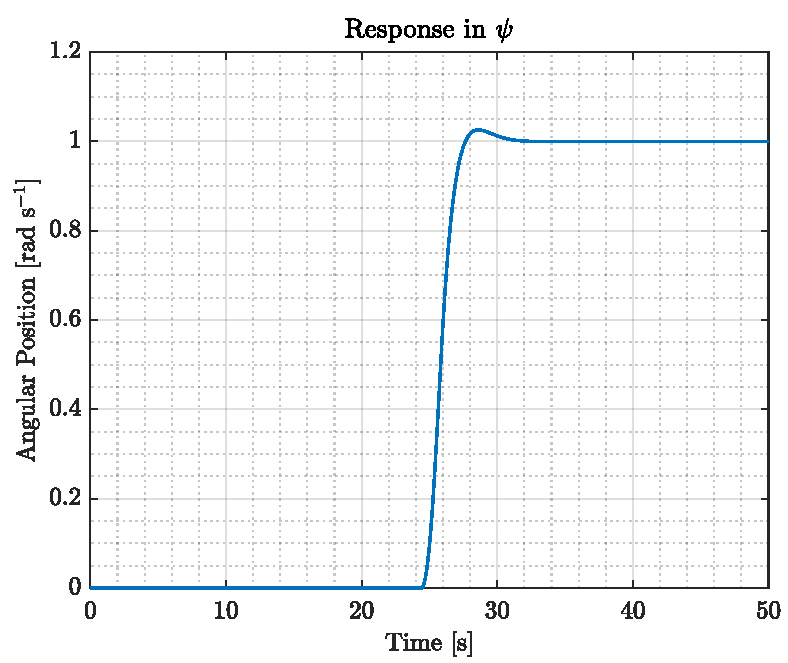
\includegraphics[width=.45\textwidth]{figures/model_node_yaw}         
    }                                                                    
    \hspace{5pt}                                                  
    \captionbox
    {    
        Step response in $\dot{x}_\mathrm{b}$ of the implemented controller code for the inner controller together with the model node.    
        \label{fig:model_node_xbdot}                               
    }                                                                  
    {                                                                    
        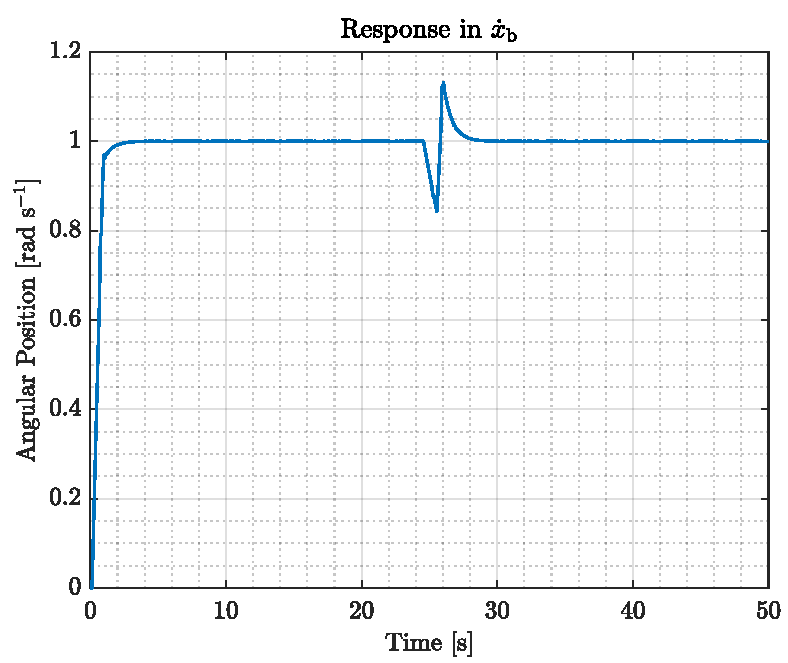
\includegraphics[width=.45\textwidth]{figures/model_node_xbdot}         
    }                                                                         
\end{figure}

\begin{figure}[H]
    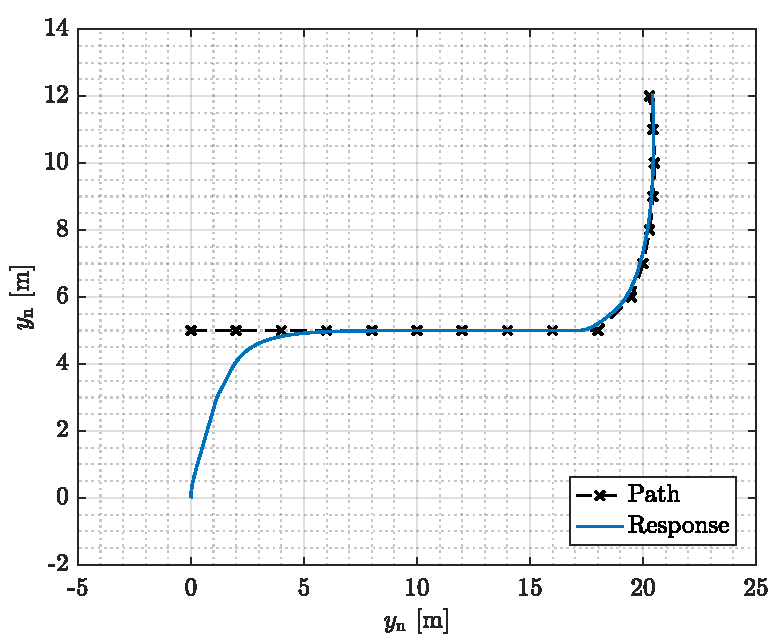
\includegraphics[width=.45\textwidth]{figures/model_node_path}
    \caption{Path and response of the implemented code, both the inner and the outer controllers together with the model node.}
    \label{fig:model_node_path}
\end{figure}

As it can be seen, both $\psi$ and $\dot{x}_\mathrm{b}$ converge to the reference when using the inner controller and the model follows the path when using the outer one. This proves that both controller nodes work and are coded properly.